\documentclass{article}         % other are available, like book
\pagestyle{empty}
\usepackage{float}
\usepackage{amssymb}            % adds more math symbols
\usepackage{amsmath}            % adds more math symbols
\usepackage[pdftex]{graphicx}
\setlength{\topmargin}{-.5in}
\setlength{\textheight}{9.0in}
\setlength{\textwidth}{6.5in}
\setlength{\oddsidemargin}{0.00in}
\setlength{\evensidemargin}{0.00in}
\setlength{\parindent}{0.0cm}	% Don't indent the paragraphs
\setlength{\parskip}{0.0cm}	% distance between paragraphs
\setlength{\abovedisplayskip}{0pt}
\begin{document}
\flushright
Chris Wozny\\
\today\\
ECE579E\\
Homework 5\\
\flushleft

\textbf{Theory of Operation:} For this assignment, we were tasked with creating a simple single cycle processor capable of the following instructions:\\

\begin{figure}[H]
\begin{center}
\begin{tabular}{ |c|c|l| }\hline
  \textbf{Opcode} & \textbf{Instruction} & \textbf{Comments} \\\hline
  000 & LDA & Load accumulator from memory\\\hline
  001 & STA & Store accumulator in memory\\\hline
  010 & ADD & Add value in memory to accumulator \\\hline
  011 & SUB & Subtract value in memory from accumulator \\\hline
  100 & JMP & Unconditional direct jump \\\hline
  101 & JEZ & Direct jump when accumulator is zero \\\hline
  110 & LDI & Load accumulator immediately, sign extend \\\hline
  111 & HLT & Halt execution until reset \\\hline
\end{tabular}
\end{center}
\end{figure}

\textbf{Design:} The design was modeled after the example given in class. The schematic is shown below and the modules are described below it:\\

\begin{figure}[H]
\begin{center}
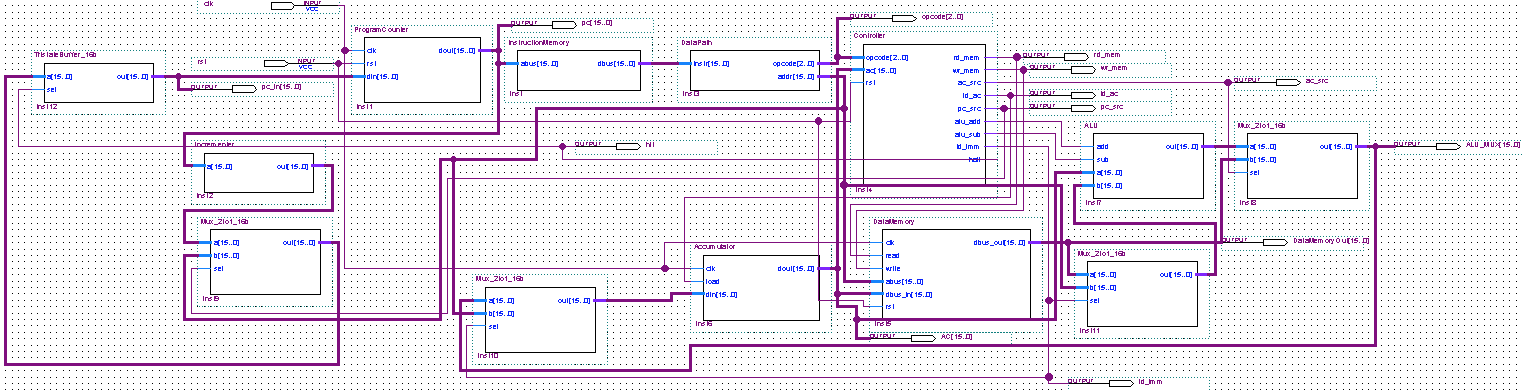
\includegraphics[scale=0.3]{schematic.png}\\
\end{center}
\caption{Schematic for Single Cycle CPU}
\end{figure}

\textbf{ALU}: Adds or subtracts the two inputs based on the select line.\\
\textbf{Accumulator:} Stores value on the positive edge of the clock when the $load$ line is high.\\
\textbf{Controller:} Uses opcode to determine the values of the following lines: $rd\_mem$, $wr\_mem$, $ac\_src$, $ld\_ac$, $ld\_imm$, $pc\_src$, $alu\_add$, $alu\_sub$, and $halt$.\\
\textbf{Data Memory:} Stores an array of 16-bit data which is initially zero'd out.\\
\textbf{Data Path:} Takes the instruction as an input and passes the opcode and address as outputs.\\
\textbf{Incrementer:} Adds one to the current input.\\
\textbf{Instruction Memory:} Holds the instructions to be executed by the processor.\\
\textbf{2-to-1 16-bit Mux:} Multiplexer which passes through input value specified by the select line.\\
\textbf{Program Counter:} Loads value from input and outputs that value. This controls which instruction in memory will be executed.\\
\textbf{Tristate Passthrough:} Passes through the 16-bit input value if the select line is low. If the select line is high, the output will be high impedance.\\

\newpage

\textbf{Simulation:} The waveform below shows the following sequence of instruction calls:
\begin{verbatim}
LDI A // load the value A immediately into the accumulator
STA 0 // store the value of the accumulator into memory address 0
LDI 4 // load the value 4 immediately into the accumulator
STA 1 // store the value of the accumulator into memory address 1
LDI 1 // load the value 1 immediately into the accumulator
STA 2 // store the value of the accumulator into memory address 2
LDA 0 // load the value at memory address 0 into the accumulator
ADD 2 // add the value at memory address 2 to the accumulator
STA 0 // store the value of the accumulator into memory address 0
LDA 1 // load the value at memory address 1 into the accumulator
SUB 2 // subtract the value at memory address 2 from the accumulator
STA 1 // store the value in the accumulator into memory address 1
JEZ E // if value in accumulator is 0, move PC to instruction memory address 14
JMP 6 // move the PC to instruction memory address 6
HLT // halt execution of processor until reset
\end{verbatim}

\begin{figure}[H]
\begin{center}
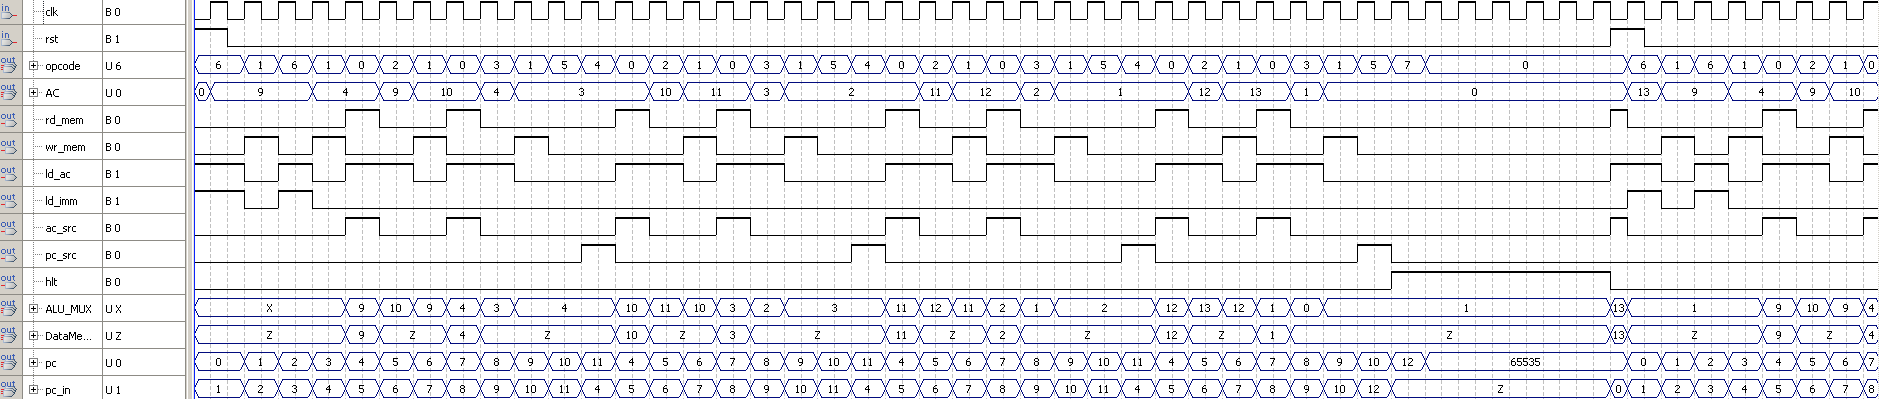
\includegraphics[scale=0.29]{waveform.png}\\
\end{center}
\caption{Output from Single Cycle CPU}
\end{figure}

In the waveform above, you can see the accumulator being loaded with the value 9 and then stored into memory address 0. Then the accumulator is loaded with the value 4 and then store it into memory address 1. After this 1 is loaded into the accumulator and stored in memory address 2. Memory address 0 is loaded into the accumulator and incremented then stored back into the same memory address. Memory address 1 is then loaded into the accumulator and decremented and stored back into memory address 1. This continues until the accumulator is 0 and then is sent into the halt state where no instructions are executed and no memory is modified. Then the reset line is pulled high and the sequence described above is restarted.\\

\newpage

\textbf{Conclusion:} In conclusion, the single cycle CPU performs as expected. Due to time constraints, the portion of the assignment which asked to write a Verilog testbench which translated mnemonics to machine code and executed them was unable to be completed. In order to test the execution of the assembly code, the InstructionMemory.v file needs to be modified and the instructions can be listed in the $mem$ array as 16-bit machine code.

\end{document}
